\section{Results}
In this section we report the statistical analysis according to the research questions of the study.

\subsection{Data Exploration}
In order to obtain a general understanding of the collected data, we first summarize the descriptive statistics of energy consumption grouped by two target applications in terms of the whole dataset in Table 6. Considering the parametric statistics, Spotify outperforms YouTube Music. When it comes to the mean consumed energy, Spotify (160.2 J) is 17.2\% lower than YouTube Music (193.5 J). Similarly, the median energy consumption of Spotify (156.9 J) is 20.2\% less than the one of YouTube Music (194.6 J). 

\begin{table}[t]
\centering
\caption{Descriptive statistics of energy consumption (Joules) per app}
\label{table1}
\begin{tabular}{|c|c|c|c|c|c|c|}
\hline
 & \textbf{Min}  & \textbf{\makecell{1st \\ Qu.}} & \textbf{Median} & \textbf{Mean} & \textbf{\makecell{3nd \\ Qu.}} & \textbf{Max}
 \\
\hline

\textbf{Spotify} & 106.3           
&154.3
&156.9
&160.2
&161.1
&212.3
\\ 
\hline

\textbf{\makecell{YouTube \\ Music}} & 144.5           
&194.6
&196.7
&193.5
&199.6
&220.8

\\ 
\hline


\end{tabular}
\label{table_MAP}
\end{table}

Since our main research question can be further boiled down into 3 sub-questions, we also perform statistical analyses on different factors including connection type, sound volume, and audio quality. The results are listed in Table 7 and Table 8, accompanied by a set of box plots for each subdataset. In this way, we offer a thorough overview of the impact that different variables have. It is interesting to note that a substantial amount of outliers are detected in all box plots. This phenomenon might be due to the existence of numerous identical records and is discussed in detail in Section 7 and Section 8. Since they are not wrongly measured data, we keep these outliers for the sake of completeness. 

\textbf{Connection Type}: Given the play mode, we distinguish between Wi-Fi streaming and downloaded file playing. Figure 3 shows the distribution of energy consumption in Spotify and YouTube Music, respectively. There exists a clear difference with regard to application, which matches the overall trend of the entire dataset. Specifically, Spotify is less energy-consuming than YouTube Music in both connection types. Despite the fact that the average energy consumption of Wi-Fi streaming (162.0 J for Spotify and 194.6 J for YouTube Music) exceeds the one of downloaded file playing (157.9 J for Spotify and 192.5 J for YouTube Music), the variance of two treatments are trivially small.

\begin{figure}[htbp]
 \centering
 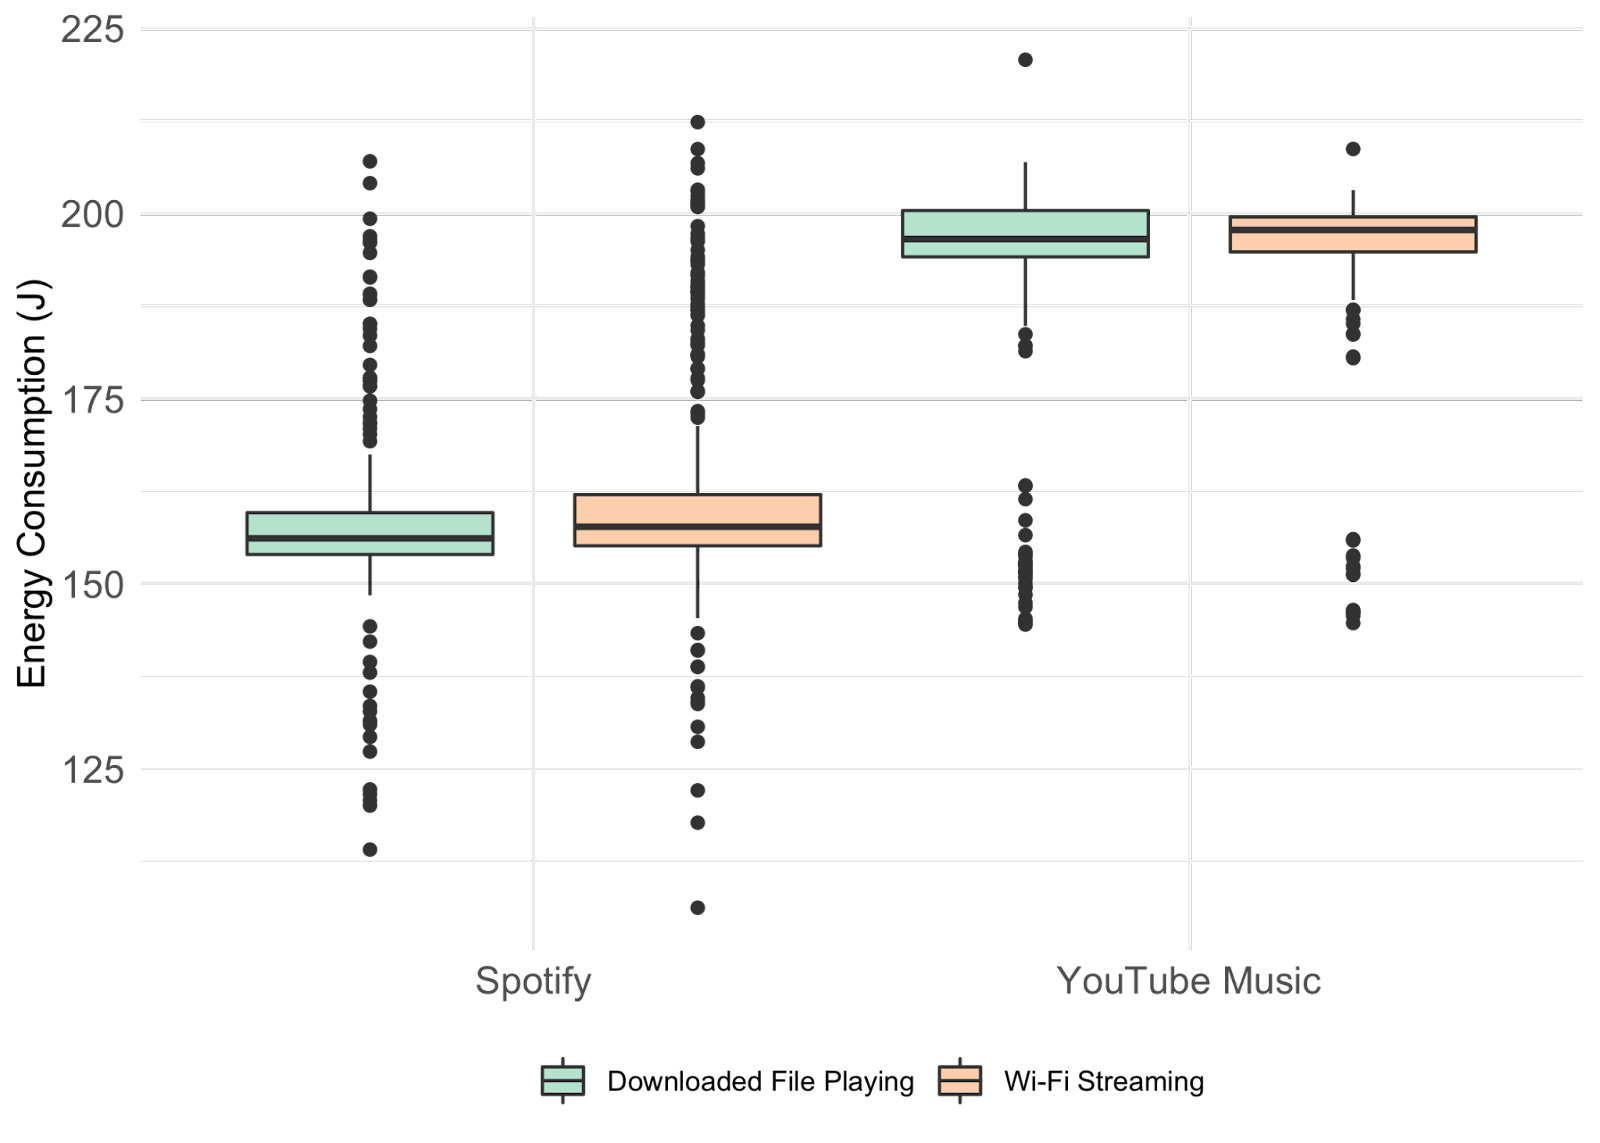
\includegraphics[width=0.8\linewidth]{reportTemplate/figures/Figure 3.png}\caption{Box plot of energy consumption (J) for RQ1.1 connection type per app}
\end{figure}

\textbf{Sound Volume}: Figure 3 and Figure 4 have in common that they both illustrate a large difference between experiments that were conducted in Spotify and the ones in YouTube Music. However, except for the high volume, box plots of low and medium volume are nearly identical. The range of energy consumption at these two levels for both applications is negligible: Both Spotify (from 158.4 J to 159.6 J) and YouTube Music (from 192.7 J to 193.6 J) experience a less than 1\% mean increase. 

From the perspective of maximum, it is noteworthy that both applications embrace abnormal data points. For Spotify, the maximum energy consumed at low volume (206.8 J) is even greater than the one at medium volume (203.2 J). Similarly, the maximal value of medium volume in YouTube Music ranks the first (220.8 J), followed by low volume (208.7 J) and high volume (206.4 J). Given the condensed data and extreme outliers, we assume that other factors like connection type and audio quality have more significant impact on the energy consumption. 

\begin{figure}[htbp]
 \centering
 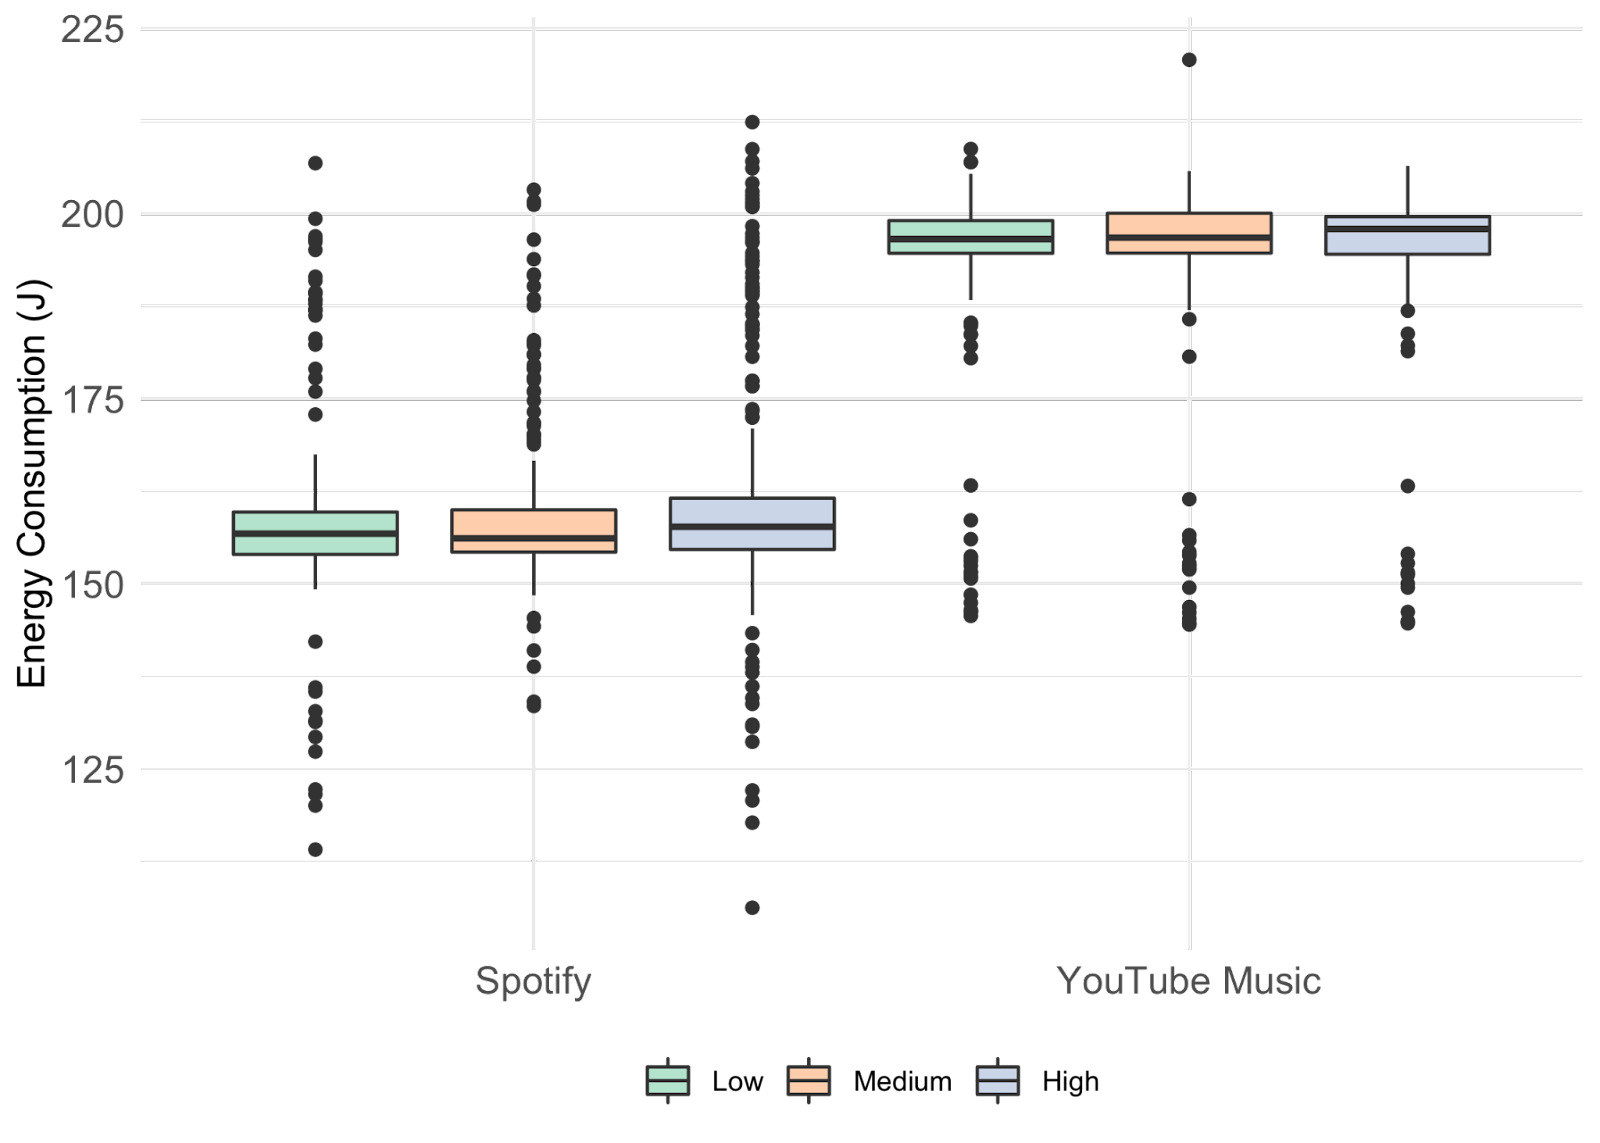
\includegraphics[width=0.8\linewidth]{reportTemplate/figures/Figure 4.png}\caption{Box plot of energy consumption (J) for RQ1.2 sound volume per App}
\end{figure}

\textbf{Audio Quality}: Though YouTube Music provides “high” audio quality, it automatically switches between all options depending on the Internet condition. In other words, the behavior of “high” audio quality brings unpredictable results. This is why we exclude it from treatments. In Figure 5, the energy consumption of the highest audio quality in both applications takes the lead, and the rest of them consume a similar amount of energy. Turning on to the very high audio quality in Spotify costs 162.9 J whereas YouTube Music consumes even more (198.2 J). 

\begin{figure}[htbp]
 \centering
 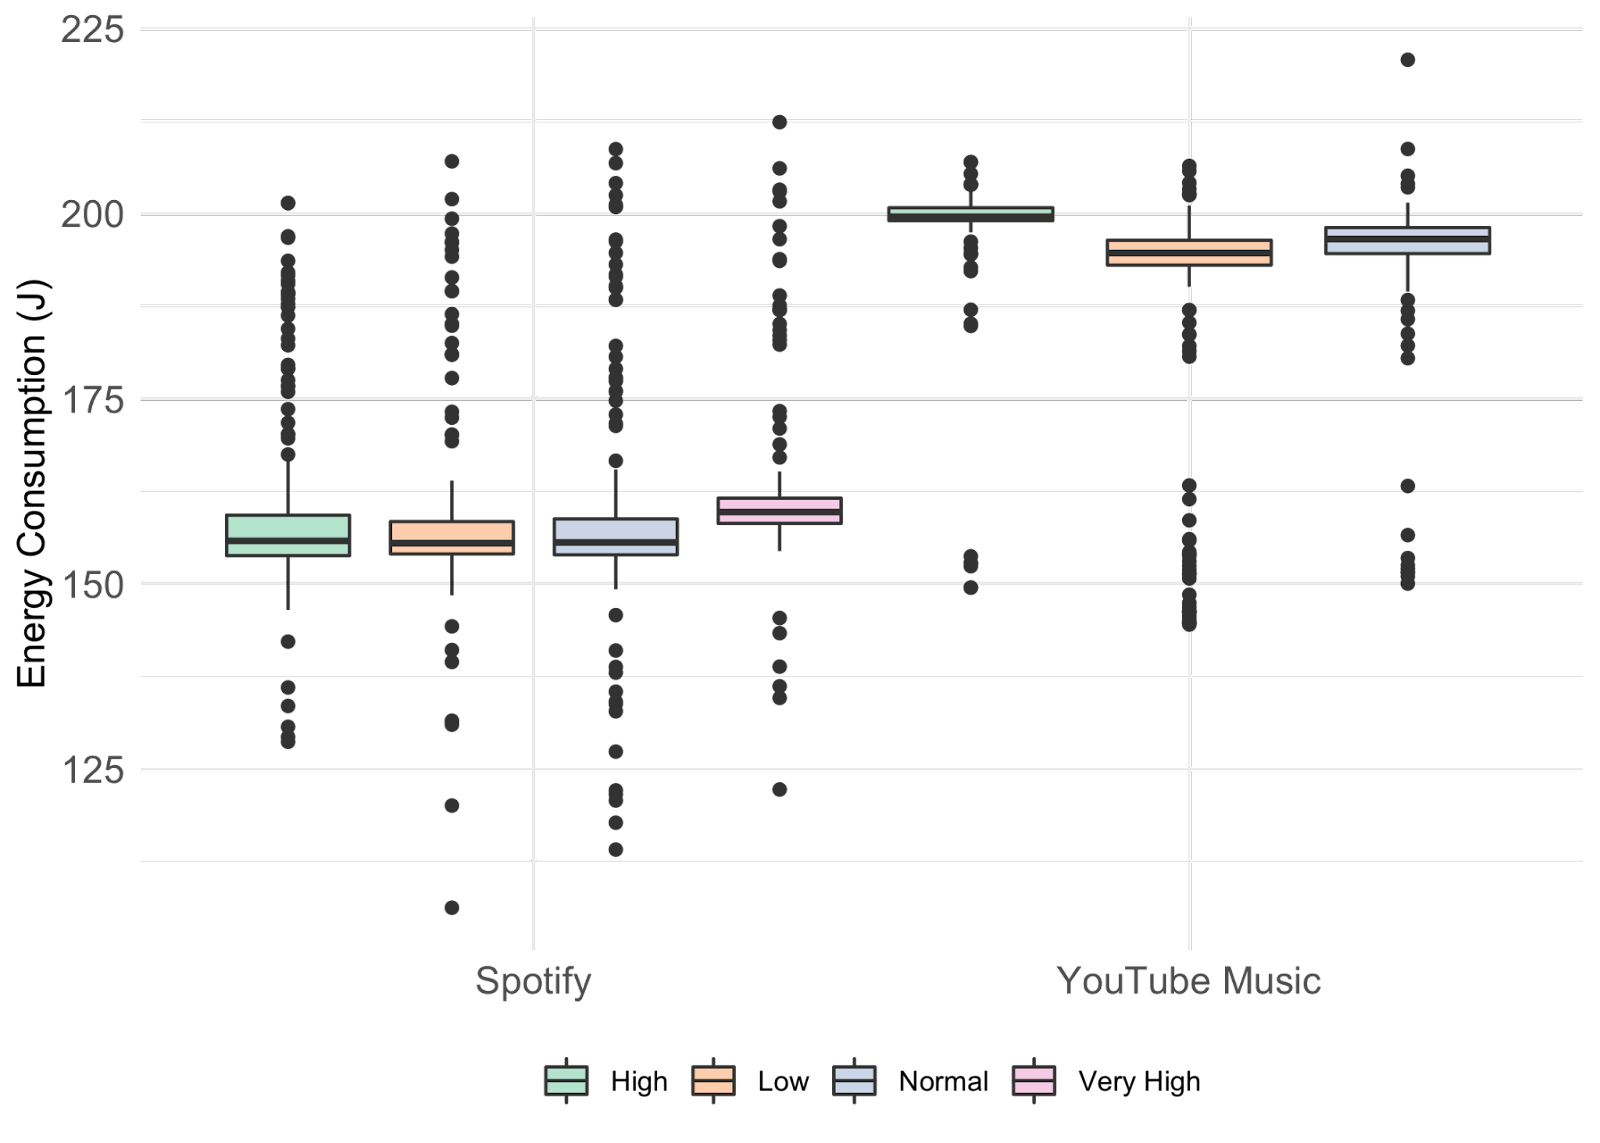
\includegraphics[width=0.8\linewidth]{reportTemplate/figures/Figure 5.png}\caption{Box plot of energy consumption (J) for RQ1.3 audio quality per app}
\end{figure}

\begin{table*}[t]
\centering
\caption{Energy consumption (Joules) for Spotify}
\label{table1}
\begin{tabular}{|c|c|c|c|c|c|c|c|}
\hline
\multirow{2}{*}{\textbf{Variable}}  & \multirow{2}{*}{\textbf{Treatment}} &  \multicolumn{6}{c|}{\textbf{Energy Consumption (Joules)}}\\
\cline{3-8}
& & \textbf{Min}& \textbf{1st Qu.} & \textbf{Median} & \textbf{Mean} & \textbf{3nd Qu.} & \textbf{Max}

\\
\hline

\multirow{2}{*}{\textbf{Connection Type}}  & \textbf{Wi-Fi Streaming} &  106.3
&155.1
&157.7
&162.0
&157.2
&212.3
\\
\cline{2-8}
&\textbf{Downloaded File Playing}
&114.1
&153.9
&156.1
&157.9
&159.6
&207.0
\\
\hline

\multirow{2}{*}{\textbf{Sound Volume}}  & \textbf{Low} &  
114.1
&154.0
&156.8
&158.4
&159.7
&206.8

\\
\cline{2-8}
&\textbf{Medium}
&133.5
&154.3
&156.1
&159.6
&160.0
&203.2
\\
\cline{2-8}
&\textbf{High}
&106.3
&154.6
&157.7
&162.5
&161.6
&212.3

\\
\hline

\multirow{2}{*}{\textbf{Audio Quality}}  & \textbf{Low} &  
106.3
&154.0
&155.5
&158.6
&158.4
&207.0

\\
\cline{2-8}
&\textbf{Normal}
&114.1
&153.9
&155.6
&159.3
&158.8
&208.7

\\
\cline{2-8}
&\textbf{High}
&128.7           
&153.8
&155.8
&160.0
&159.3
&201.4

\\
\cline{2-8}
&\textbf{Very High}
&122.2   
&158.1 
&159.7  
&162.9   
&161.6   
&212.3

\\
\hline

\end{tabular}
\label{table_MAP}
\end{table*}

\begin{table*}[t]
\centering
\caption{Energy consumption (Joules) for YouTube Music}
\label{table1}
\begin{tabular}{|c|c|c|c|c|c|c|c|}
\hline
\multirow{2}{*}{\textbf{Variable}}  & \multirow{2}{*}{\textbf{Treatment}} &  \multicolumn{6}{c|}{\textbf{Energy Consumption (Joules)}}\\
\cline{3-8}
& & \textbf{Min}& \textbf{1st Qu.} & \textbf{Median} & \textbf{Mean} & \textbf{3nd Qu.} & \textbf{Max}

\\
\hline

\multirow{2}{*}{\textbf{Connection Type}}  & \textbf{Wi-Fi Streaming} &  144.7
&194.8
&197.8
&194.6
&199.5
&208.7

\\
\cline{2-8}
&\textbf{Downloaded File Playing}
&144.5
&194.1
&196.5
&192.5
&200.4
&220.8

\\
\hline

\multirow{2}{*}{\textbf{Sound Volume}}  & \textbf{Low} &  
145.7
&194.6
&196.5
&192.7
&199.0
&208.7

\\
\cline{2-8}
&\textbf{Medium}
&144.5
&194.7
&196.7
&193.6
&200.0
&220.8

\\
\cline{2-8}
&\textbf{High}
&144.7
&194.5
&197.9
&194.4
&199.6
&206.4

\\
\hline

\multirow{2}{*}{\textbf{Audio Quality}}  & \textbf{Low} &  
144.5
&193.0
&194.7
&187.9
&196.4
&206.4

\\
\cline{2-8}
&\textbf{Normal}
&150.0
&194.6
&196.5
&194.6
&198.1
&220.8

\\
\cline{2-8}
&\textbf{Always High}
&149.5
&199.0
&199.6
&198.2
&200.8
&206.9

\\
\hline

\end{tabular}
\label{table_MAP}
\end{table*}



\subsection{Normality Testing}
Considering the continuous dependent variable (\ie energy consumption) and independent samples, the next step is to check the normality of data distribution. We first inspect the density plot and Q-Q plot to obtain an initial indication about the normality, and then apply the Shapiro-Wilk test as a complementary approach to validating the conclusion. If the dataset is normally distributed, it should encompass the following characteristics: (1) Density plot displays the bell-shaped curve, (2) Q-Q plot shows a diagonal straight line, and (3) p-value of the Shapiro-Wilk test should be greater than 0.05. 

Figure 6 presents an overview of statistical distribution of the energy consumed in each run for Spotify and YouTube Music. One can identify two distinct peaks of frequent values in each application (roughly 160 J for Spotify and 195 J for YouTube Music). Hence, it not only corroborates the observations that Spotify is less energy-hungry than YouTube Music but implies that the data are asymmetrical owing to the skewness. What’s more, the Q-Q plot does not show a diagonal straight line. Last but not the least, p-values ($p<2.2e - 16$) of the Shapiro-Wilk test for both apps are lower than the significance threshold. To conclude, we have enough evidence to reject the null hypothesis that the dataset is normally distributed. 

\begin{figure}[htbp]
 \centering
 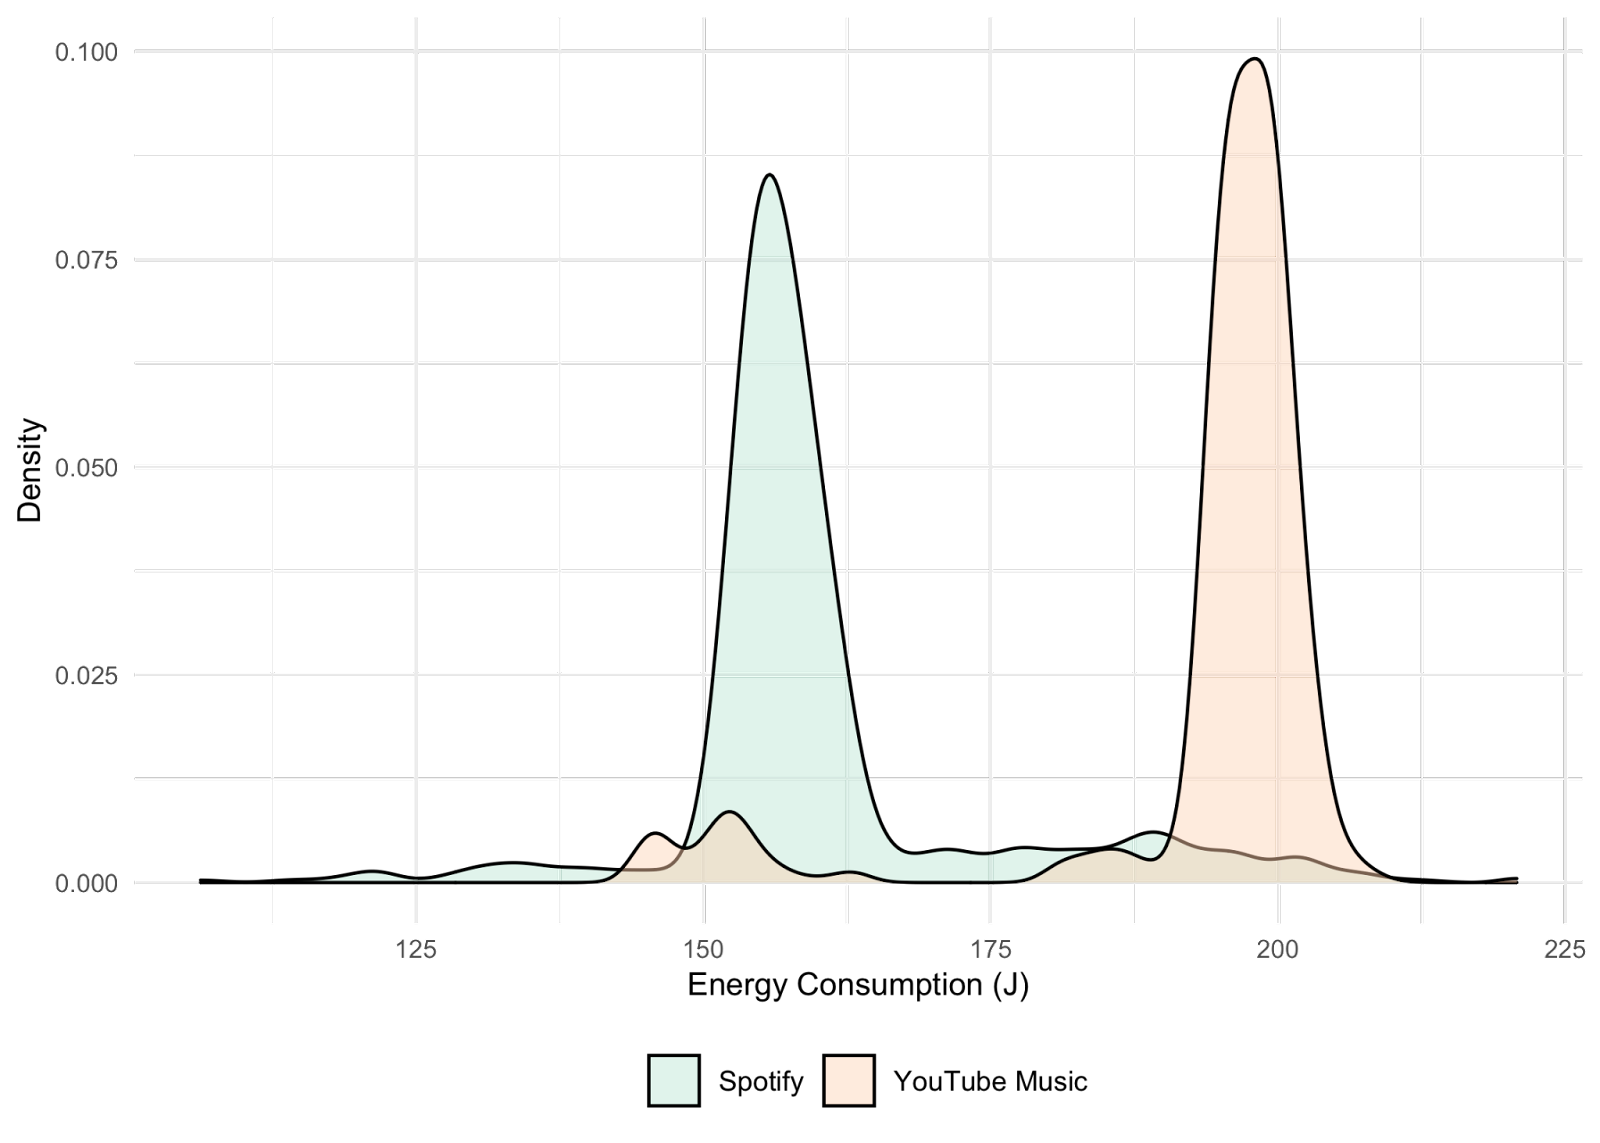
\includegraphics[width=0.8\linewidth]{reportTemplate/figures/Figure 6.png}\caption{Density plot of energy consumption (J) per app}
\end{figure}

\begin{figure}[htbp]
 \centering
 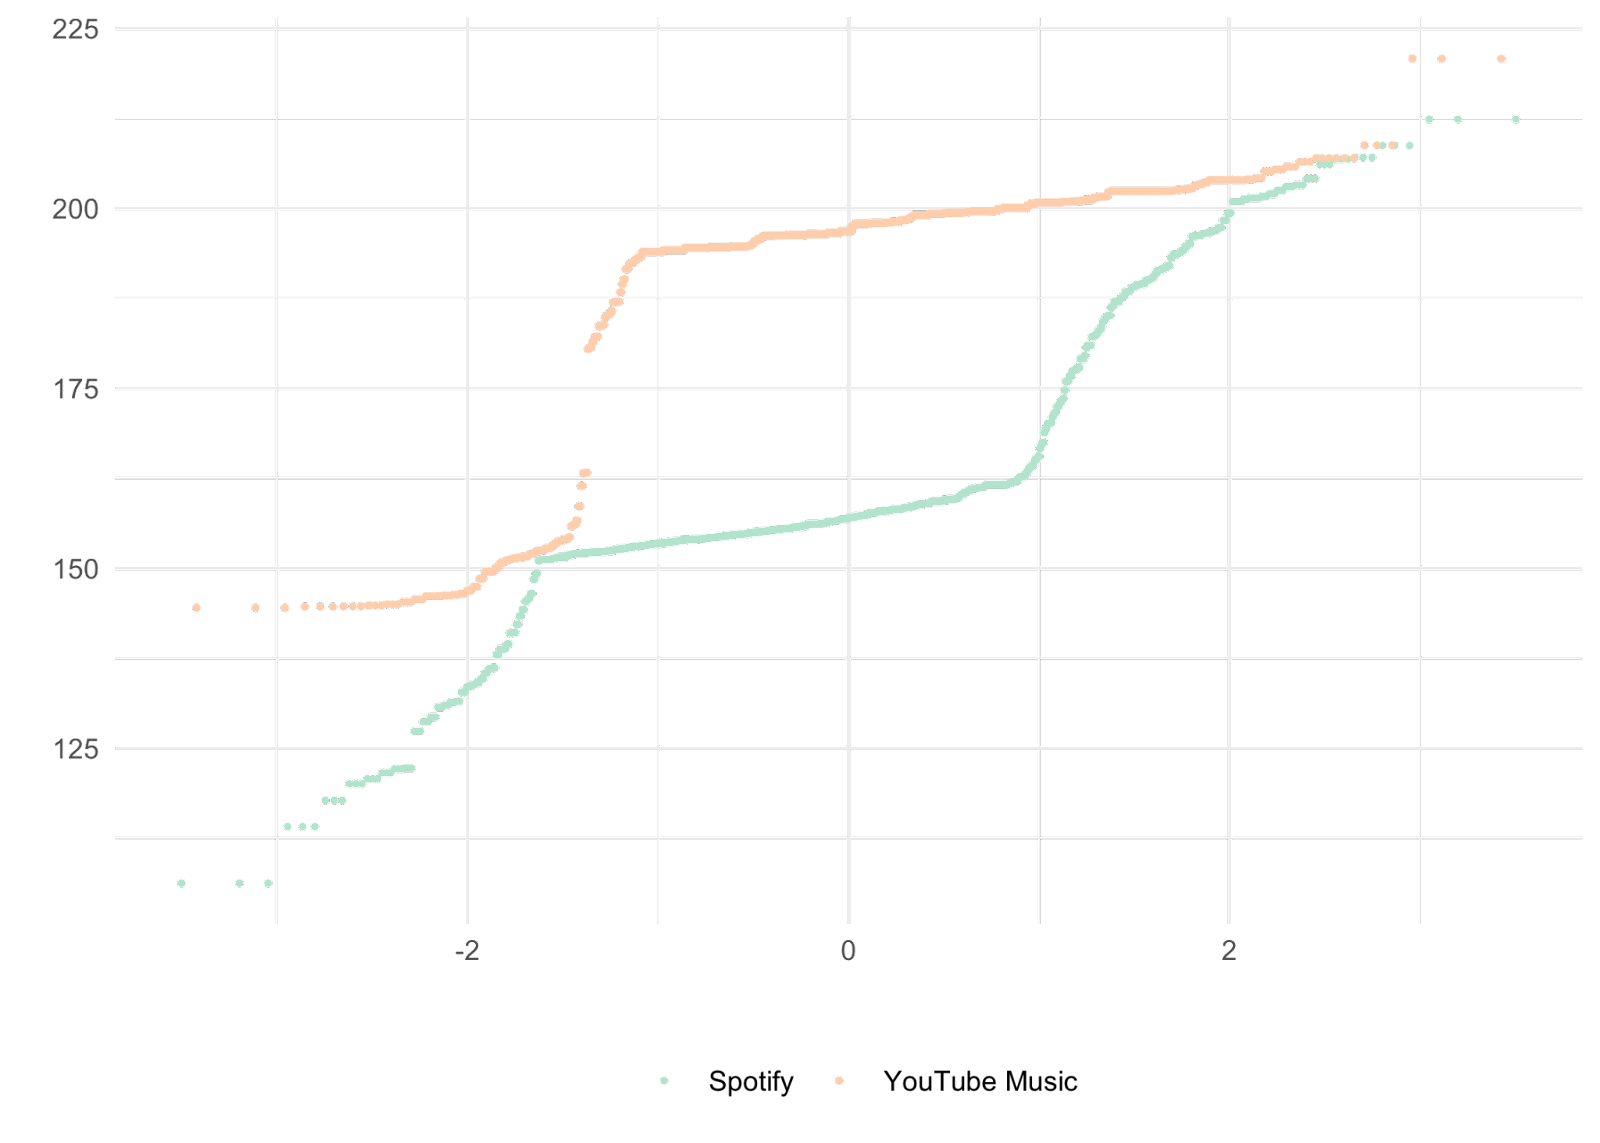
\includegraphics[width=0.8\linewidth]{reportTemplate/figures/Figure 7.png}\caption{Density plot of energy consumption (J) per app}
\end{figure}

Taking one step further, we partition the dataset to check the data normality in order to investigate sub-questions. Figure 8 and Figure 9 provide a fine-grained view of the distribution grouped by treatments. Furthermore, Table 9 lists all p-values in terms of treatment and most of them are smaller than $2.2e - 16$. The combined result confirms the previous findings that the dataset is not normally distributed for both applications.  

\begin{figure}[htbp]
 \centering
 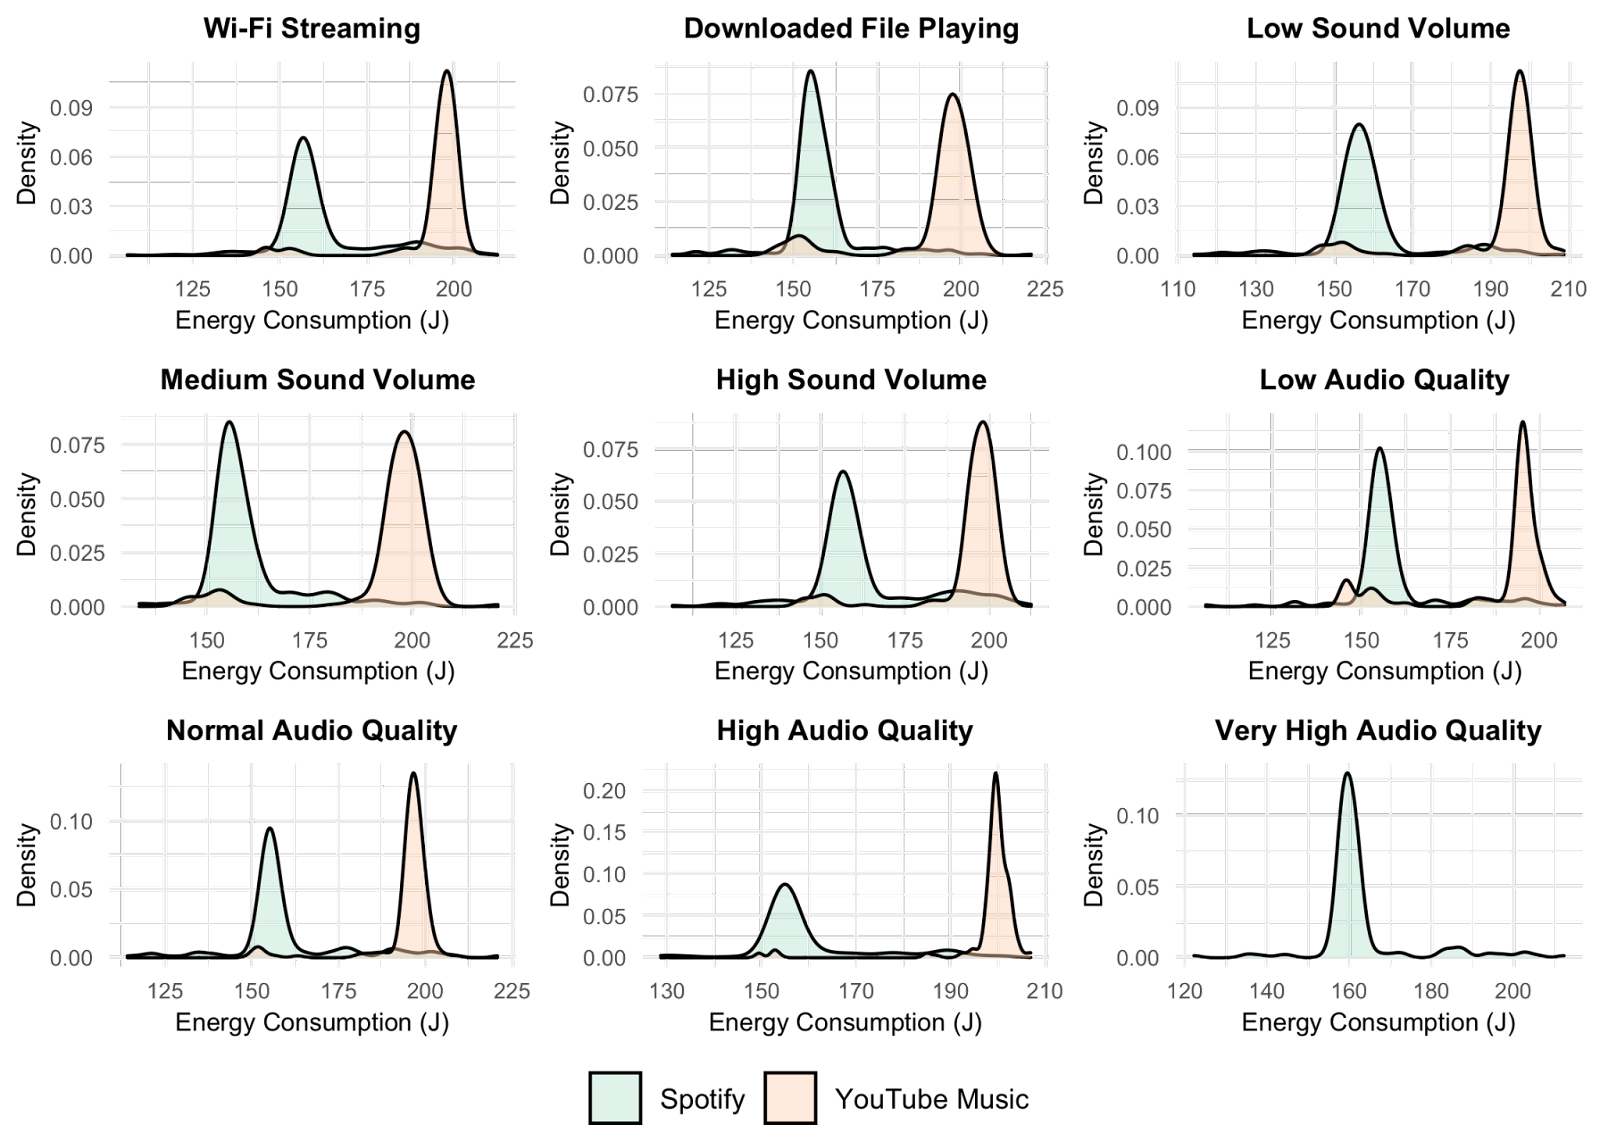
\includegraphics[width=0.8\linewidth]{reportTemplate/figures/Figure 8.png}\caption{Density plot of energy consumption (J) classified by treatments in two apps}
\end{figure}

\begin{figure}[htbp]
 \centering
 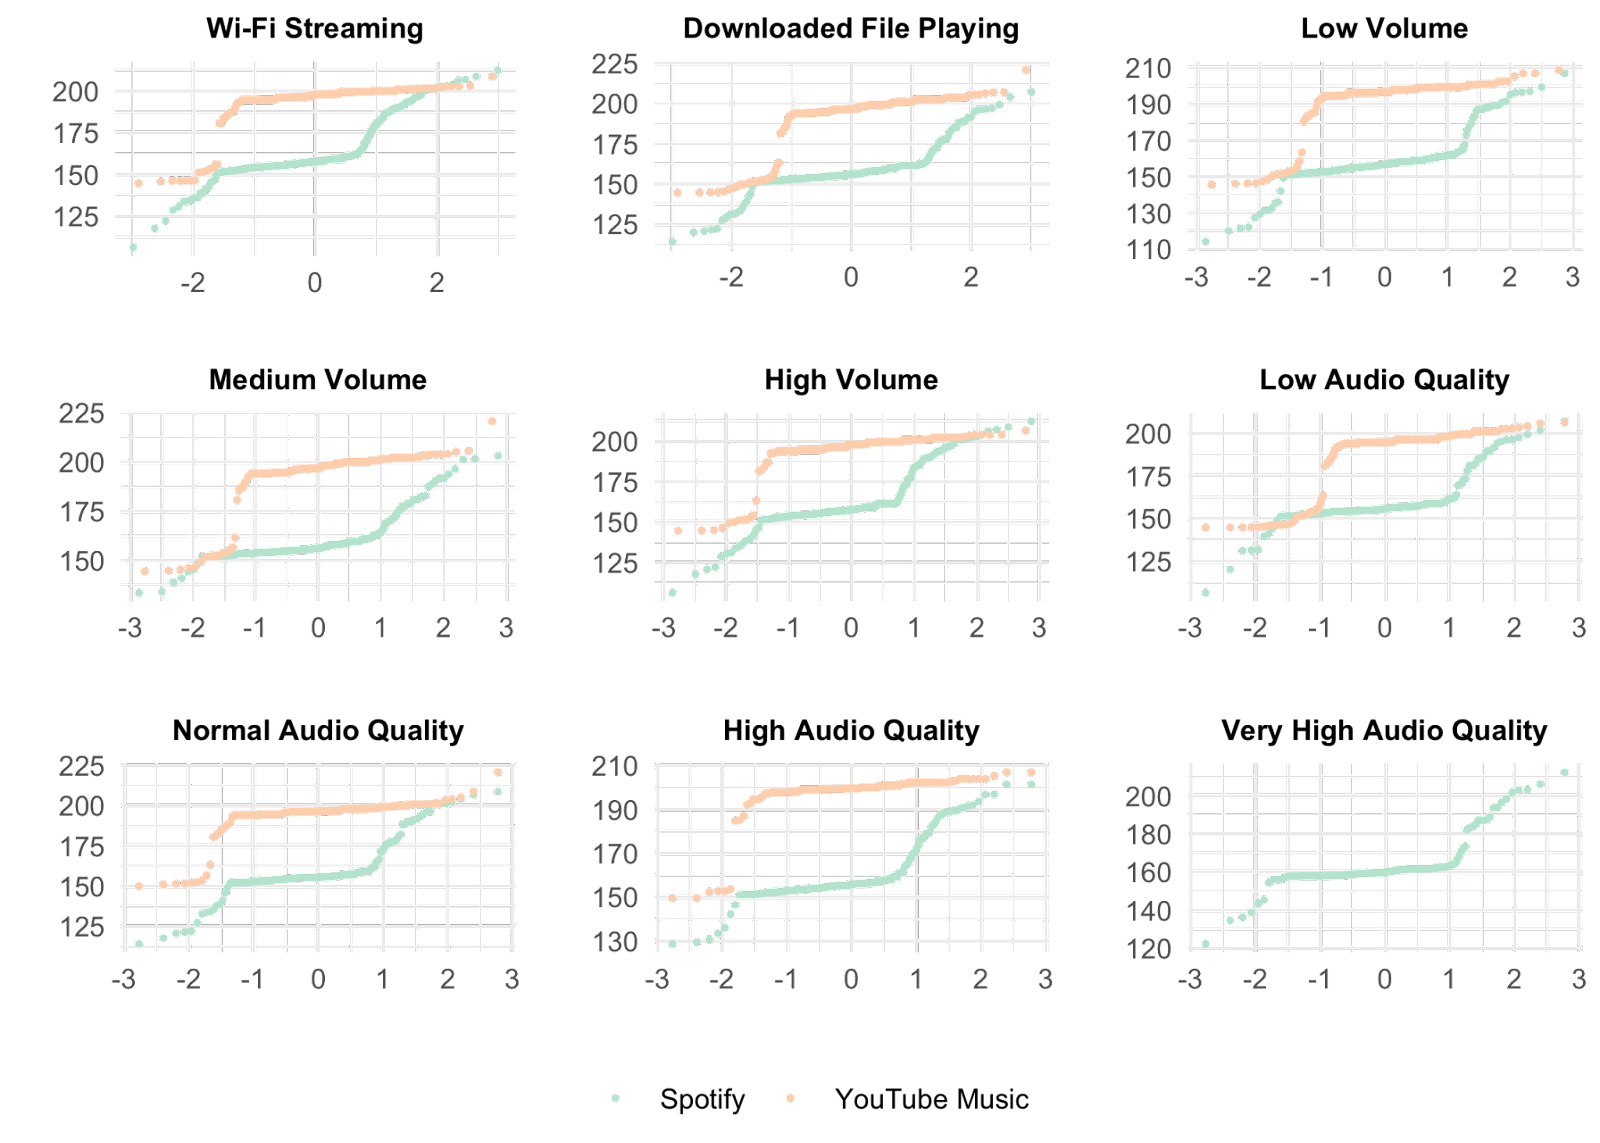
\includegraphics[width=0.8\linewidth]{reportTemplate/figures/Figure 9.png}\caption{Q-Q plot of energy consumption (J) classified by treatments in two apps}
\end{figure}

\begin{table}[t]
\centering
\caption{ p-value using the Shapiro-Wilk test for different treatments}
\label{table1}
\begin{tabular}{|c|c|c|c|}
\hline
\multirow{2}{*}{\textbf{Variable}}  & \multirow{2}{*}{\textbf{Treatment}} &  \multicolumn{2}{c|}{\textbf{p-value}}\\
\cline{3-4}
& & \textbf{Spotify}& \textbf{\makecell{YouTube \\Music} }
\\
\hline

\multirow{2}{*}{\textbf{\makecell{Connection \\ Type}}}  & \textbf{\makecell{Wi-Fi \\ Streaming}} &  
< 2.2e-16
&< 2.2e-16


\\
\cline{2-4}
&\textbf{\makecell{Downloaded \\ File Playing}}
&< 2.2e-16
&< 2.2e-16
\\
\hline

\multirow{2}{*}{\textbf{\makecell{Sound \\ Volume}}}  & \textbf{Low} &  
< 2.2e-16
&< 2.2e-16

\\
\cline{2-4}
&\textbf{Medium}
&< 2.2e-16
&< 2.2e-16
\\
\cline{2-4}
&\textbf{High}
&5.701e-15
&< 2.2e-16

\\
\hline

\multirow{2}{*}{\textbf{\makecell{Audio\\ Quality}}}  & \textbf{Low} &  
< 2.2e-16
&< 2.2e-16

\\
\cline{2-4}
&\textbf{Normal}
&1.495e-14
&< 2.2e-16

\\
\cline{2-4}
&\textbf{(Always) High}
&1.848e-15
&< 2.2e-16

\\
\cline{2-4}
&\textbf{Very High}
&< 2.2e-16
& -

\\
\hline

\end{tabular}
\label{table_MAP}
\end{table}

\subsection{Hypothesis Testing}

Given the fact that datasets fail to pass the normality checking, we implement the non-parametric tests to answer all research (sub-) questions by means of testing the null hypotheses proposed in Section 4.3. Due to the different number of factors, research questions fall into two categories, namely one-factor-two-treatments (RQ1 - 1.1) and one-factor-multiple-treatments (RQ1.2 - 1.3). Therefore, different non-parametric tests are applied accordingly: the Mann-Whitney test is applied for RQ1 - 1.1 whereas the Kruskal-Wallis test for RQ1.2 - 1.3. In addition, with the purpose of mitigating the false discovery rate, especially caused by Type I errors, the Benjamini–Hochberg procedure is employed to adjust a series of p-values.  

For RQ1 - 1.1, Table 10 documents p-values and adjusted p-values generated by the Mann-Whitney test and the Benjamini–Hochberg procedure, respectively. Except for H1.$1_0$ regarding the connection type in YouTube Music, p-values of all other hypotheses are below the threshold of significance (\ie 0.05). Therefore, we have confidence in rejecting the null hypothesis H$1_0$ and H1.$1_0$ for Spotify. In other words, there exists a significant statistical difference between Spotify and YouTube Music in terms of energy consumption. In addition, connection type has a significant impact on the consumed energy in Spotify. Different from Spotify, whether to use Wi-Fi streaming or not does not result in the variance of energy consumption in YouTube Music.


\begin{table*}[t]
\centering
\caption{p-values using the Mann-Whitney test and adjusted p-values using the Benjamini–Hochberg procedure for RQ1 - 1.1}
\begin{threeparttable}
\label{table1}
\begin{tabular}{|c|c|c|c|c|c|}
\hline
\multirow{2}{*}{\textbf{Hypothesis}}  &
\multirow{2}{*}{\textbf{Treatment}} & \multicolumn{2}{c|}{\textbf{p-value}} & \multicolumn{2}{c|}{\textbf{Adjusted p-value}}\\
\cline{3-6}

 & & Spotify & YouTube Music & Spotify & YouTube Music

 \\
\hline

H1_0 & Spotify vs. YouTube Music & \multicolumn{2}{c|}{\textbf{< 2.2e-16}} &\multicolumn{2}{c|}{\textbf{9.9000000e-16}}
 \\
\hline

H1.1_0 & Connection Type & \textbf{5.934e-06} &0.4652& \textbf{1.038455e-05} & 0.4652
 \\ 
\hline


\end{tabular}
\label{table_MAP}
 \begin{tablenotes}
        \footnotesize
        \item * p-value < 0.05 (\ie reject the null hypothesis) is marked in bold 
      \end{tablenotes}
  \end{threeparttable}
\end{table*}
For RQ1.2 - 1.3, p-values produced by the Kruskal-Wallis test as well as its adjustment are shown in Table 11. On the one hand, as p-value (0.09388) is greater than 0.05, we cannot reject the null hypothesis H1.$2_0$ in regard to YouTube Music, which means that we cannot claim that different volume levels contribute to the distinct energy consumption. In contrast, as for Spotify, we can reject the null hypothesis H1.$2_0$ and assert that the volume level does influence the consumed energy. On the other hand, H1.$3_0$ of both applications get rejected and we have strong evidence to state that audio quality poses an indispensable impact on energy consumption. 

\begin{table*}[t]
\centering
\caption{p-values using the Kruskal-Wallis test and adjusted p-values using the Benjamini–Hochberg procedure for RQ1.2 - 1.3}
\begin{threeparttable}
\label{table1}
\begin{tabular}{|c|c|c|c|c|c|}
\hline
\multirow{2}{*}{\textbf{Hypothesis}}  &
\multirow{2}{*}{\textbf{Treatment}} & \multicolumn{2}{c|}{\textbf{p-value}} & \multicolumn{2}{c|}{\textbf{Adjusted p-value}}\\
\cline{3-6}

 & & Spotify & YouTube Music & Spotify & YouTube Music

 \\
\hline

H1.$2_0$ & Sound Volume & \textbf{0.01223}
&0.09388
&\textbf{1.712006e-02}
&0.09388
 \\
\hline

H1.$3_0$ & Audio Quality & \textbf{< 2.2e-16} & 
\textbf{< 2.2e-16} & 
\textbf{5.411765e-24} & 
\textbf{1.631714e-36} 
 \\ 
\hline


\end{tabular}
\label{table_MAP}
 \begin{tablenotes}
        \footnotesize
        \item * p-value < 0.05 (\ie reject the null hypothesis) is marked in bold 
      \end{tablenotes}
  \end{threeparttable}
\end{table*}

In order to identify the factor that poses a greater impact on the energy consumption, post-hoc Dunn’s test is conducted for the non-parametric pairwise multiple comparison between group levels. Due to the prerequisite of a significant Kruskal-Wallis test, we exclude the H1.$2_0$ for YouTube Music. The results documented in Table 12 and Table 13 correspond to the box plots in Section 6.1 to a great extent: as for Spotify, apart from pairs consisting of the greatest value (\ie high volume or very high audio quality), the remaining treatments do not distinguish between each other. Nevertheless, all treatment groups regarding audio quality in YouTube Music exhibit a statistically significant difference.

\begin{table}[t]
\centering
\caption{\centering p-values using the Dunn’s test \protect\\for H1.\bm{${2_0}$} (Spotify only)}
\begin{threeparttable}
\label{table1}
\begin{tabular}{|c|c|}
\hline
\textbf{Treatment Group} & \textbf{p-value}\\
\hline

Low Volume $\sim$ Medium Volume
&0.720

\\ 
\hline

Low Volume $\sim$ High Volume
&\textbf{0.00632}

\\
\hline

Medium Volume $\sim$ High Volume
&0.0177

 \\
\hline

\end{tabular}
\label{table_MAP}
 \begin{tablenotes}
        \footnotesize
        \item * p-value < 0.05 (\ie reject the null hypothesis) is marked in bold 
      \end{tablenotes}
  \end{threeparttable}
\end{table}

\begin{table}[t]
\centering
\caption{p-values using the Dunn’s test for H1.\bm{${3_0}$}}
\begin{threeparttable}
\label{table1}
\begin{tabular}{|c|c|c|}
\hline
\textbf{Treatment Group} & \multicolumn{2}{c|}{\textbf{p-value}}\\
\cline{2-3}

&Spotify&YouTube Music
\\ 
\hline
\makecell{High Audio Quality $\sim$ \\Low Audio Quality}
&0.6
&\textbf{1.27e-36}

\\
\hline

\makecell{High Audio Quality $\sim$ \\Normal Audio Quality}
&0.885
&\textbf{3.39e-18}

 \\
\hline

\makecell{High Audio Quality $\sim$  \\Very High Audio Quality}
&\textbf{2.90e-17}
&- 
\\
\hline
\makecell{Low Audio Quality $\sim$ \\Normal Audio Quality}
&0.704
&\textbf{8.06e-5}
\\
\hline
\makecell{Low Audio Quality $\sim$ \\ Very High Audio Quality}
&\textbf{2.83e-19}
&-
\\
\hline
\makecell{Normal Audio Quality $\sim$ \\Very High Audio Quality}
&\textbf{8.33e-18}
&-
\\
\hline


\end{tabular}
\label{table_MAP}
 \begin{tablenotes}
        \footnotesize
        \item * p-value < 0.05 (\ie reject the null hypothesis) is marked in bold 
      \end{tablenotes}
  \end{threeparttable}
\end{table}

\subsection{Effect Size Estimation }
As a quantitative measure of the magnitude of different effect that each factor poses on energy consumption, effect size facilitates the evaluation of the strength of a phenomenon. As explained in Section 4.5, the larger the effect size, the stronger the relationship between independent and dependent variables. 

In light of differnt types of statistical tests, distinct effect size estimation methods are applied, namely the Cliff’s delta for the Mann-Whitney test (\ie RQ1 - 1.1) while the Eta-squared for the Kruskal-Wallis test (\ie RQ1.2 - 1.3). Table 14 and Table 15 list all research questions’ effect sizes and their classification. To begin with, the overall comparison between Spotify and YouTube Music produces a large effect size of 0.80. The effect size of connection type and sound volume in both applications are small or negligible. On the contrary, the effect size of audio quality is large. To summarize, compared to connection type and sound volume, audio quality is more likely to be the dominant factor that determines the energy consumption. 

\begin{table}[t]
\centering
\caption{\centering Effect size estimation using the Cliff’s delta \protect\\for RQ1 - 1.1}
\label{table1}
\begin{tabular}{|c|c|c|c|}
\hline
\multirow{2}{*}{\textbf{\makecell{Research \\Question}}}  &\multirow{2}{*}{\textbf{Treatment}} & \multicolumn{2}{c|}{\textbf{Effect Size
}}\\
\cline{3-4}

 & &\textbf{Spotify} & \textbf{\makecell{YouTube\\ Music}} \\
\hline

RQ1 & \makecell{Spotify vs. \\YouTube Music}& \multicolumn{2}{c|}{\makecell{0.803948 (Large)}}
\\ 
\hline

RQ1.1 & 
\makecell{Connection 
\\
Type}
&
\makecell{0.1950231 
\\
(Small)}
&
\makecell{0.03632373 
\\
(Negligible)}

 \\
\hline

\end{tabular}
\label{table_MAP}
\end{table}

\begin{table}[t]
\centering
\caption{\centering Effect size estimation using the eta-squared \protect\\for RQ1.2 - 1.3}
\label{table1}
\begin{tabular}{|c|c|c|c|}
\hline
\multirow{2}{*}{\textbf{\makecell{Research \\Question}}}  &\multirow{2}{*}{\textbf{Treatment}} & \multicolumn{2}{c|}{\textbf{Effect Size
}}\\
\cline{3-4}

 & &\textbf{Spotify} & \textbf{\makecell{YouTube \\ Music}} \\
\hline

RQ1.2
&Sound Volume
&0.00950 (Small)
&0.00509 (Small)
\\
\hline
RQ1.3
&Audio Quality
&0.154 (Large)
&0.308 (Large)

\\
\hline

\end{tabular}
\label{table_MAP}
\end{table}